\section{Kiến trúc hệ thống}
    \begin{figure}[h]
        \centering
        \includegraphics[width=0.6\linewidth]{Images/Roadside.png}
        \caption{Kiến trúc hệ thống}
    \end{figure}

% % \section{Kiến trúc mạng}
% % \begin{figure}[h]
% %         \centering
% %         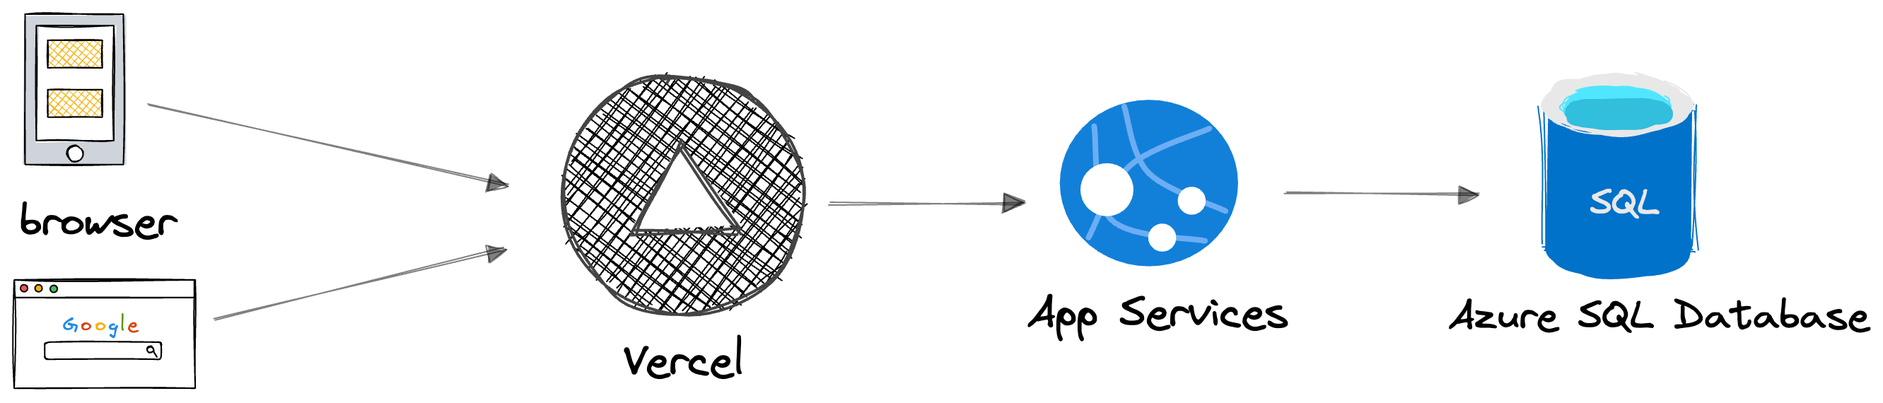
\includegraphics[width=0.8\linewidth]{Images/network.png}
% %         \vspace{1em}
% %         \caption{Kiến trúc mạng}
% %         \label{fig:enter-label}
% %     \end{figure}

% % Kiến trúc này được triển khai để kết nối giữa người dùng cuối, nền tảng triển khai ứng dụng, và cơ sở dữ liệu. Các thành phần chính trong kiến trúc bao gồm:
% % \begin{itemize}
% %     \item \textbf{Browser (Trình duyệt):} Trình duyệt web và các thiết bị di động là điểm bắt đầu, nơi người dùng tương tác với ứng dụng web. Người dùng truy cập vào ứng dụng thông qua giao diện web, thực hiện các thao tác như đăng nhập, tìm kiếm, và quản lý thông tin.
% %     \item \textbf{Vercel:} Vercel là nền tảng triển khai ứng dụng được sử dụng trong hệ thống này. Nó đảm bảo việc phân phối nội dung tĩnh và động một cách nhanh chóng và hiệu quả. Vercel chịu trách nhiệm triển khai và quản lý mã nguồn của ứng dụng web, đảm bảo rằng các yêu cầu từ phía người dùng được xử lý kịp thời và hiệu quả. Vercel nhận các yêu cầu từ trình duyệt, xử lý chúng và tương tác với các dịch vụ back-end để lấy dữ liệu cần thiết.
% %     \item \textbf{App Services:} App Services đóng vai trò là server của hệ thống. Nó thực hiện các logic nghiệp vụ của ứng dụng, tương tác với cơ sở dữ liệu để xử lý và lưu trữ dữ liệu cần thiết. Các dịch vụ này chịu trách nhiệm xử lý các yêu cầu từ Vercel, thực hiện các tác vụ như xác thực người dùng, xử lý dữ liệu, và thực thi các quy trình nghiệp vụ của ứng dụng. App Services kết nối trực tiếp với cơ sở dữ liệu Azure SQL Database để truy xuất và cập nhật dữ liệu.
% %     \item \textbf{Azure SQL Database:} Azure SQL Database là cơ sở dữ liệu chính của hệ thống. Nó chịu trách nhiệm lưu trữ và quản lý tất cả dữ liệu cần thiết cho ứng dụng. Cơ sở dữ liệu này đảm bảo tính toàn vẹn và bảo mật của dữ liệu, cung cấp khả năng truy xuất dữ liệu nhanh chóng và hiệu quả cho các dịch vụ ứng dụng. Dữ liệu từ App Services được lưu trữ và truy vấn trực tiếp từ Azure SQL Database, đảm bảo rằng mọi thông tin được lưu giữ an toàn và có thể truy cập nhanh chóng khi cần thiết.
    
% % \end{itemize}

% % Kiến trúc này đảm bảo rằng các thành phần trong hệ thống hoạt động cùng nhau một cách nhịp nhàng và hiệu quả. Trình duyệt và thiết bị di động của người dùng tương tác với Vercel, nền tảng triển khai ứng dụng, để gửi và nhận dữ liệu. Vercel đóng vai trò trung gian, chuyển tiếp các yêu cầu đến App Services, nơi thực hiện các logic nghiệp vụ và xử lý dữ liệu. App Services sau đó tương tác với Azure SQL Database để truy xuất và lưu trữ dữ liệu cần thiết, đảm bảo rằng hệ thống hoạt động mượt mà, hiệu quả và an toàn.\\

% % Kiến trúc này không chỉ đảm bảo khả năng mở rộng và linh hoạt cho ứng dụng mà còn cung cấp một môi trường bảo mật và hiệu quả cho việc quản lý và xử lý dữ liệu. Sự kết hợp giữa các công nghệ hiện đại như Vercel, Azure App Services, và Azure SQL Database tạo ra một hệ thống mạnh mẽ, đáng tin cậy và dễ dàng bảo trì trong tương lai.

% \section{API Endpoints}

% \subsection{App Settings}

% \subsubsection*{/api/settings - GET}
% \begin{tabular}{|>{\raggedright\arraybackslash}p{3cm}|p{12cm}|}
% \hline
% \textbf{Operation} & GET \\
% \hline
% \textbf{Description} & Retrieve application settings. \\
% \hline
% \textbf{Responses} & 200: Success \\
% \hline
% \end{tabular}

% \subsubsection*{/api/settings - POST}
% \begin{tabular}{|>{\raggedright\arraybackslash}p{3cm}|p{12cm}|}
% \hline
% \textbf{Operation} & POST \\
% \hline
% \textbf{Description} & Create new application setting. \\
% \hline
% \textbf{Request Body} & AppSettings schema (JSON) \\
% \hline
% \textbf{Responses} & 200: Success \\
% \hline
% \end{tabular}

% \subsubsection*{/api/settings - DELETE}
% \begin{tabular}{|>{\raggedright\arraybackslash}p{3cm}|p{12cm}|}
% \hline
% \textbf{Operation} & DELETE \\
% \hline
% \textbf{Description} & Delete a specific setting based on ID. \\
% \hline
% \textbf{Parameters} & id: string (required) \\
% \hline
% \textbf{Responses} & 200: Success \\
% \hline
% \end{tabular}

% \subsubsection*{/api/settings/update - POST}
% \begin{tabular}{|>{\raggedright\arraybackslash}p{3cm}|p{12cm}|}
% \hline
% \textbf{Operation} & POST \\
% \hline
% \textbf{Description} & Update multiple settings in a single request. \\
% \hline
% \textbf{Request Body} & Array of AppSettings schema (JSON) \\
% \hline
% \textbf{Responses} & 200: Success \\
% \hline
% \end{tabular}

% \subsection{Authentication}

% \subsubsection*{/api/auth/signup - POST}
% \begin{tabular}{|>{\raggedright\arraybackslash}p{3cm}|p{12cm}|}
% \hline
% \textbf{Operation} & POST \\
% \hline
% \textbf{Description} & Register a new account. \\
% \hline
% \textbf{Request Body} & Account schema (JSON) \\
% \hline
% \textbf{Responses} & 200: Success \\
% \hline
% \end{tabular}

% \subsubsection*{/api/auth/login - POST}
% \begin{tabular}{|>{\raggedright\arraybackslash}p{3cm}|p{12cm}|}
% \hline
% \textbf{Operation} & POST \\
% \hline
% \textbf{Description} & Authenticate a user and return a token. \\
% \hline
% \textbf{Request Body} & LoginInfo schema (JSON) \\
% \hline
% \textbf{Responses} & 200: Success \\
% \hline
% \end{tabular}

% \subsubsection*{/api/auth/logout - POST}
% \begin{tabular}{|>{\raggedright\arraybackslash}p{3cm}|p{12cm}|}
% \hline
% \textbf{Operation} & POST \\
% \hline
% \textbf{Description} & Log out a user and invalidate the session token. \\
% \hline
% \textbf{Responses} & 200: Success \\
% \hline
% \end{tabular}

% \subsection{Orders}

% \subsubsection*{/api/orders - GET}
% \begin{tabular}{|>{\raggedright\arraybackslash}p{3cm}|p{12cm}|}
% \hline
% \textbf{Operation} & GET \\
% \hline
% \textbf{Description} & Retrieve all orders. \\
% \hline
% \textbf{Responses} & 200: Success \\
% \hline
% \end{tabular}

% \subsubsection*{/api/orders - POST}
% \begin{tabular}{|>{\raggedright\arraybackslash}p{3cm}|p{12cm}|}
% \hline
% \textbf{Operation} & POST \\
% \hline
% \textbf{Description} & Create a new order. \\
% \hline
% \textbf{Request Body} & Orders schema (JSON) \\
% \hline
% \textbf{Responses} & 200: Success \\
% \hline
% \end{tabular}

% \subsubsection*{/api/orders - DELETE}
% \begin{tabular}{|>{\raggedright\arraybackslash}p{3cm}|p{12cm}|}
% \hline
% \textbf{Operation} & DELETE \\
% \hline
% \textbf{Description} & Delete a specific order based on ID. \\
% \hline
% \textbf{Parameters} & id: string (required) \\
% \hline
% \textbf{Responses} & 200: Success \\
% \hline
% \end{tabular}

% \subsubsection*{/api/orders/voucher - GET}
% \begin{tabular}{|>{\raggedright\arraybackslash}p{3cm}|p{12cm}|}
% \hline
% \textbf{Operation} & GET \\
% \hline
% \textbf{Description} & Retrieve all vouchers associated with orders. \\
% \hline
% \textbf{Responses} & 200: Success \\
% \hline
% \end{tabular}

% \subsubsection*{/api/orders/voucher - DELETE}
% \begin{tabular}{|>{\raggedright\arraybackslash}p{3cm}|p{12cm}|}
% \hline
% \textbf{Operation} & DELETE \\
% \hline
% \textbf{Description} & Delete a voucher based on the given ID. \\
% \hline
% \textbf{Parameters} & id: string (required) \\
% \hline
% \textbf{Responses} & 200: Success \\
% \hline
% \end{tabular}

% \subsubsection*{/api/orders/items - GET}
% \begin{tabular}{|>{\raggedright\arraybackslash}p{3cm}|p{12cm}|}
% \hline
% \textbf{Operation} & GET \\
% \hline
% \textbf{Description} & Retrieve all items in all orders. \\
% \hline
% \textbf{Responses} & 200: Success \\
% \hline
% \end{tabular}

% \subsubsection*{/api/orders/items - DELETE}
% \begin{tabular}{|>{\raggedright\arraybackslash}p{3cm}|p{12cm}|}
% \hline
% \textbf{Operation} & DELETE \\
% \hline
% \textbf{Description} & Delete an item from an order based on the given ID. \\
% \hline
% \textbf{Parameters} & id: string (required) \\
% \hline
% \textbf{Responses} & 200: Success \\
% \hline
% \end{tabular}

% \subsubsection*{/api/orders/update - POST}
% \begin{tabular}{|>{\raggedright\arraybackslash}p{3cm}|p{12cm}|}
% \hline
% \textbf{Operation} & POST \\
% \hline
% \textbf{Description} & Update multiple orders in a single request. \\
% \hline
% \textbf{Request Body} & Array of Orders schema (JSON) \\
% \hline
% \textbf{Responses} & 200: Success \\
% \hline
% \end{tabular}

% \subsection{Products}

% \subsubsection*{/api/products - GET}
% \begin{tabular}{|>{\raggedright\arraybackslash}p{3cm}|p{12cm}|}
% \hline
% \textbf{Operation} & GET \\
% \hline
% \textbf{Description} & Retrieve all products with details. \\
% \hline
% \textbf{Responses} & 200: Success, returns an array of products. \\
% \hline
% \end{tabular}

% \subsubsection*{/api/products - POST}
% \begin{tabular}{|>{\raggedright\arraybackslash}p{3cm}|p{12cm}|}
% \hline
% \textbf{Operation} & POST \\
% \hline
% \textbf{Description} & Create a new product entry with detailed specifications. \\
% \hline
% \textbf{Request Body} & Products schema (JSON) \\
% \hline
% \textbf{Responses} & 200: Success, product created. \\
% \hline
% \end{tabular}

% \subsubsection*{/api/products - DELETE}
% \begin{tabular}{|>{\raggedright\arraybackslash}p{3cm}|p{12cm}|}
% \hline
% \textbf{Operation} & DELETE \\
% \hline
% \textbf{Description} & Delete a specific product based on product ID. \\
% \hline
% \textbf{Parameters} & id: string (required) \\
% \hline
% \textbf{Responses} & 200: Success, product deleted. \\
% \hline
% \end{tabular}

% \subsubsection*{/api/products/search - GET}
% \begin{tabular}{|>{\raggedright\arraybackslash}p{3cm}|p{12cm}|}
% \hline
% \textbf{Operation} & GET \\
% \hline
% \textbf{Description} & Search for products by name. \\
% \hline
% \textbf{Parameters} & name: string (required) \\
% \hline
% \textbf{Responses} & 200: Success, returns matching products. \\
% \hline
% \end{tabular}

% \subsubsection*{/api/products/{id} - GET}
% \begin{tabular}{|>{\raggedright\arraybackslash}p{3cm}|p{12cm}|}
% \hline
% \textbf{Operation} & GET \\
% \hline
% \textbf{Description} & Retrieve detailed information about a product by ID. \\
% \hline
% \textbf{Parameters} & id: string (required) \\
% \hline
% \textbf{Responses} & 200: Success, returns product details. \\
% \hline
% \end{tabular}

% \subsubsection*{/api/products/categories - GET}
% \begin{tabular}{|>{\raggedright\arraybackslash}p{3cm}|p{12cm}|}
% \hline
% \textbf{Operation} & GET \\
% \hline
% \textbf{Description} & Retrieve all product categories. \\
% \hline
% \textbf{Responses} & 200: Success, returns categories array. \\
% \hline
% \end{tabular}

% \subsubsection*{/api/products/categories - DELETE}
% \begin{tabular}{|>{\raggedright\arraybackslash}p{3cm}|p{12cm}|}
% \hline
% \textbf{Operation} & DELETE \\
% \hline
% \textbf{Description} & Delete a specific category based on category ID. \\
% \hline
% \textbf{Parameters} & id: string (required) \\
% \hline
% \textbf{Responses} & 200: Success, category deleted. \\
% \hline
% \end{tabular}

% \subsubsection*{/api/products/prices - GET}
% \begin{tabular}{|>{\raggedright\arraybackslash}p{3cm}|p{12cm}|}
% \hline
% \textbf{Operation} & GET \\
% \hline
% \textbf{Description} & Retrieve pricing information for all products. \\
% \hline
% \textbf{Responses} & 200: Success, returns prices array. \\
% \hline
% \end{tabular}

% \subsubsection*{/api/products/prices - DELETE}
% \begin{tabular}{|>{\raggedright\arraybackslash}p{3cm}|p{12cm}|}
% \hline
% \textbf{Operation} & DELETE \\
% \hline
% \textbf{Description} & Delete pricing information based on price ID. \\
% \hline
% \textbf{Parameters} & id: string (required) \\
% \hline
% \textbf{Responses} & 200: Success, price information deleted. \\
% \hline
% \end{tabular}

% \subsubsection*{/api/products/update - POST}
% \begin{tabular}{|>{\raggedright\arraybackslash}p{3cm}|p{12cm}|}
% \hline
% \textbf{Operation} & POST \\
% \hline
% \textbf{Description} & Update multiple product entries in a single request. \\
% \hline
% \textbf{Request Body} & Array of Products schema (JSON) \\
% \hline
% \textbf{Responses} & 200: Success, products updated. \\
% \hline
% \end{tabular}

% % \subsection{Stripe Integration}

% % \subsubsection*{/api/stripe/customer/add - POST}
% % \begin{tabular}{|>{\raggedright\arraybackslash}p{3cm}|p{12cm}|}
% % \hline
% % \textbf{Operation} & POST \\
% % \hline
% % \textbf{Description} & Adds a new customer to Stripe with credit card details. \\
% % \hline
% % \textbf{Request Body} & Includes Email, Name, and Credit Card details (Name, Number, Expiration, CVC). \\
% % \hline
% % \textbf{Responses} & 200: Success, returns the created Stripe customer object. \\
% % \hline
% % \end{tabular}

% % \subsubsection*{/api/stripe/payment/add - POST}
% % \begin{tabular}{|>{\raggedright\arraybackslash}p{3cm}|p{12cm}|}
% % \hline
% % \textbf{Operation} & POST \\
% % \hline
% % \textbf{Description} & Processes a payment via Stripe for a customer. \\
% % \hline
% % \textbf{Request Body} & AddStripePayment schema, includes customer ID, receipt email, and payment details. \\
% % \hline
% % \textbf{Responses} & 200: Success, returns the Stripe payment object. \\
% % \hline
% % \end{tabular}

% % \subsubsection*{/api/stripe/create-checkout-session - POST}
% % \begin{tabular}{|>{\raggedright\arraybackslash}p{3cm}|p{12cm}|}
% % \hline
% % \textbf{Operation} & POST \\
% % \hline
% % \textbf{Description} & Creates a Stripe checkout session for handling payments on the client side. \\
% % \hline
% % \textbf{Request Body} & CreateCheckoutSessionStripeRequest schema, includes product and pricing details. \\
% % \hline
% % \textbf{Responses} & 200: Success, returns session details for client-side handling. \\
% % \hline
% % \end{tabular}

% \subsection{Users}

% \subsubsection*{/api/users - GET}
% \begin{tabular}{|>{\raggedright\arraybackslash}p{3cm}|p{12cm}|}
% \hline
% \textbf{Operation} & GET \\
% \hline
% \textbf{Description} & Retrieve a list of all users. \\
% \hline
% \textbf{Responses} & 200: Success, returns an array of user objects. \\
% \hline
% \end{tabular}

% \subsubsection*{/api/users/update - POST}
% \begin{tabular}{|>{\raggedright\arraybackslash}p{3cm}|p{12cm}|}
% \hline
% \textbf{Operation} & POST \\
% \hline
% \textbf{Description} & Update multiple user profiles in a single request. \\
% \hline
% \textbf{Request Body} & Array of Users schema (JSON), allowing batch updates. \\
% \hline
% \textbf{Responses} & 200: Success, users updated. \\
% \hline
% \end{tabular}

% \subsubsection*{/api/users/account - GET}
% \begin{tabular}{|>{\raggedright\arraybackslash}p{3cm}|p{12cm}|}
% \hline
% \textbf{Operation} & GET \\
% \hline
% \textbf{Description} & Retrieve account details for the logged-in user. \\
% \hline
% \textbf{Responses} & 200: Success, returns user account details. \\
% \hline
% \end{tabular}

% \subsubsection*{/api/users/account - DELETE}
% \begin{tabular}{|>{\raggedright\arraybackslash}p{3cm}|p{12cm}|}
% \hline
% \textbf{Operation} & DELETE \\
% \hline
% \textbf{Description} & Delete a user account based on the given ID. \\
% \hline
% \textbf{Parameters} & id: string, UUID (required) \\
% \hline
% \textbf{Responses} & 200: Success, account deleted. \\
% \hline
% \end{tabular}

% % Add more tables for other endpoints as needed

